\chapter{Optimierung und Evaluierung}

Im folgenden Kapitel werden die vorgenommenen Optimierungsmaßnahmen und die damit einhergehende Evaluierung der Ergebnisse der Link Discovery beschrieben. Dazu gehören der gewählte Ansatz zur Optimierung, eine Erläuterung evolutionärer Algorithmen und deren Einsatz zur Optimierung sowie die Darstellung und Auswertung der Ergebnisse.

\section{Optimierung}

Zuerst muss definiert werden, welcher Aspekt genau optimiert werden soll. Die in Kapitel \ref{link_discovery} beschriebenen Schritte haben einen Graphen erzeugt, in dem neun verschiedene Kantentypen existieren. Diese lauten \emph{Tag-Kookkurrenz}, \emph{Klick-Kookkurrenz}, \emph{Zusammensetzung}, \emph{Zerlegung}, \emph{Wortform}, \emph{Grundform}, \emph{Synonym}, \emph{Kategorie-Kookkurrenz} und \emph{Thesaurus-Beziehung}.

Werden nun inhaltlich relevante Nachbarn zu einem gegebenen Begriff gesucht, müssen alle ausgehenden Kanten des entsprechenden Knotens nach Relevanz geordnet werden. Dazu muss jede Kante ein Kantengewicht besitzen. Die Addition aller Kantengewichte zwischen zwei Knoten stellt somit das Maß für ihre Nähe dar.

Die Kanten vom Typ Kookkurrenz besitzen bereits aufgrund der angegebenen Kookkurrenzmaße Kantengewichte. Jedoch muss hierbei festgelegt werden, welches Maß für das Kantengewicht herangezogen werden und in welchem Verhältnis zu den Gewichten anderer Kantentypen es stehen soll.

Somit hängt die Berechnung der Relevanz zwischen zwei Knoten von zwölf Parametern ab. Jedem Kantentyp muss ein Gewicht zugewiesen und außerdem muss eine Auswahl von drei Kookkurrenzmaßen getroffen werden. Die Optimierung und Evaluierung dieser berechneten Relevanz ist Gegenstand dieses Kapitels.

Die Einschätzung, ob die Ordnung der Nachbarn eine Ordnung der Relevanz zum Ausgangsbegriff darstellt, kann nicht automatisch, sondern nur von Menschen, getroffen werden. Somit stellt die Bewertung einer bestimmten Gewichtung der Kanten auch eine Evaluierung der Kantentypen dar.
Generell kann außerdem nicht davon ausgegangen werden, dass eine einmal gefundene Gewichtung der Kanten für alle Knoten des Graphen verwertbare Ergebnisse erzeugt. Daher sollte die Optimierung nicht global, sondern für jeden Knoten einzeln erfolgen. Aufgrund der hohen Knotenanzahl wurde sich hierzu auf eine stichprobenartige Auswahl der Knotenmenge beschränkt.

Durch die Notwendigkeit menschlicher Beteiligung und der großen Anzahl an Parametern ist eine Optimierung mittels des Ausprobierens aller Fälle nicht möglich. Außerdem kann die Einschätzung, welche Kantengewichtungen relevante Ergebnisse erzeugen, stark von Mensch zu Mensch variieren. Stattdessen muss zur Optimierung ein Ansatz gefunden werden, der sich einer, für den Großteil der Personen, optimalen Gewichtung möglichst nähert. 

Im Rahmen dieser Arbeit wurde aus den genannten Gründen ein Optimierungsansatz mittels interaktiver evolutionärer Algorithmen gewählt. Die Grundlagen evolutionärer Algorithmen und die gewählte Implementierung werden in den folgenden Abschnitten beschrieben.

\section{Evolutionäre Algorithmen}

Als evolutionäre Algorithmen wird eine Klasse von Optimierungsverfahren bezeichnet, deren Funktionsweise an die Evolution natürlicher Lebewesen angelehnt ist. Sie versuchen, Probleme durch die Simulation von Evolution mittels der Auswahl der erfolgreichsten Individuen zu lösen. Dabei kommen ebenfalls aus der Biologie entlehnte Mechanismen wie Mutation und Rekombination zum Einsatz, um iterativ eine Population von Lösungskandidaten zu verbessern \cite{tw2008}.

Es handelt sich um heuristische Algorithmen, die das Finden einer optimalen Lösung nicht garantieren können.

Grundsätzlich folgt das Vorgehen einem Kreislauf mit den Komponenten \emph{Evaluierung}, \emph{Selektion} und \emph{Reproduktion}. Nach Generierung einer anfänglichen Population (\emph{Initialisierung}) wird dieser Kreislauf so lange durchlaufen, bis ein vorher definiertes Abbruchkriterium eintritt. Ein Durchlauf wird als \emph{Generation} bezeichnet. Das Abbruchkriterium kann beispielsweise ein bestimmter Schwellwert für die Güte der Lösung oder eine feste Anzahl von Generationen sein. Der beschriebene Ablauf ist in Abbildung \ref{fig:evo_basic} dargestellt.

\begin{figure}
\centering
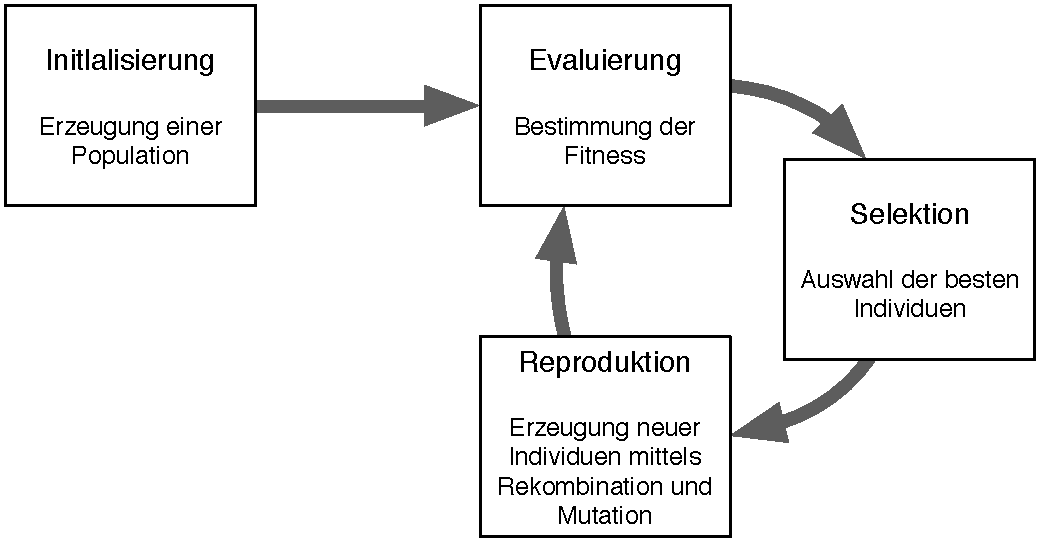
\includegraphics[width=0.8\textwidth]{evo_basic}
\caption{Ablauf evolutionärer Algorithmen}
\label{fig:evo_basic}
\end{figure}

Die einzelnen Komponenten eines evolutionären Algorithmus werden im Folgenden beschrieben. Die Definitionen folgen im Wesentlichen denen von \textcite{tw2008}.

\paragraph{Initialisierung}

Die Population \(P\) stellt eine Menge von Lösungskandidaten dar. Ein Lösungskandidat \(i\) wird als \emph{Individuum} bezeichnet und durch seinen \emph{Genotyp} repräsentiert. Der Genotyp ist die kodierte Repräsentation aller Variablen, die den Lösungskandidaten spezifizieren. Die Variablen werden \emph{Gene} genannt. Während der Initialisierung werden Lösungskandidaten erzeugt, die die Startpopulation des evolutionären Algorithmus bilden. Die Gene jedes Individuums werden üblicherweise zufällig gewählt.

\paragraph{Evaluierung}

Der Evaluierungsschritt dient zur Bestimmung der \emph{Fitness} der Individuen, die noch in der Population enthalten sind. Die Fitness stellt einen Wert dar, der die Güte der durch das Individuum repräsentierten Lösung bezüglich der Problemstellung beschreibt. Die Fitness kann, je nach Optimierungsproblem, entweder absolut oder bezüglich der anderen Individuen der Population bestimmt werden. Somit lässt sich die Funktion zur Bestimmung der Fitness auf die Form \(fitness(i, P)\) generalisieren.

\paragraph{Selektion}

Im Selektionsschritt werden die fittesten Individuen der Population ausgewählt. Alle nicht ausgewählten Lösungskandidaten werden verworfen. Die Selektion kann als Funktion der Form \(select(P, f, s)\) dargestellt werden, wobei \(s\) eine festgelegte Anzahl von Individuen darstellt, die ausgewählt werden sollen.

\paragraph{Reproduktion}

Die Reproduktion dient dazu, aus den im Selektionsschritt ausgewählten Individuen neue Lösungskandidaten zu erzeugen. Dabei werden üblicherweise die Operationen \emph{Rekombination} und \emph{Mutation} verwendet. Eine Rekombination erzeugt, analog zur Biologie, aus zwei Elternindividuen ein neues Kindindividuum. Sie lässt sich als Funktion der Form \(i_n = recombine(i_a, i_b)\) darstellen, wobei \(i_n\) das neue Individuum und \(i_a\) und \(i_b\) die Elternindividuen darstellen. Eine Mutation erzeugt ein neues Individuen durch die Modifikation eines anderen und ist daher durch die Funktion \(i_n = mutate(i_a)\) spezifiziert.

In der Literatur \cite{kw2007, tw2008, dj2006} finden sich für Selektion, Mutation und Rekombination Standardverfahren, die in Hinblick auf das zu lösende Optimierungsproblem ausgewählt werden können. Wie die beschriebenen Schritte des evolutionären Algorithmus für die Optimierung der Link Discovery implementiert wurden, wird im folgenden Abschnitt beschrieben.

\section{Umsetzung}

Nachdem im vorhergehenden Abschnitt die Grundlagen und Komponenten evolutionärer Algorithmen beschrieben wurden, werden im Folgenden die für die Optimierung der Link Discovery-Ergebnisse angewendeten Methoden erläutert.

Zunächst soll die Methode zur Auswahl der Stichproben erläutert werden. Insgesamt wurden fünfzehn Knoten ausgewählt, deren Beziehungen optimiert werden sollen. Die Auswahl der Knoten richtete sich nach der Popularität von Suchbegriffen auf der Website von Spreadshirt. Dazu wurden alle Begriffe mit mehr als eintausend Suchen herangezogen und diese nach Häufigkeit der Suchen geordnet. Daraus wurden zufällig je fünf Begriffe bis zum unteren Quartil, fünf Begriffe zwischen unterem und oberen Quartil und fünf Begriffe über dem oberen Quartil ausgewählt. Die ausgewählten Begriffe, deren Kantengewichtungen lokal optimiert werden sollen, lauten: \emph{Kopfkissenbezug}, \emph{Student}, \emph{Volkswagen}, \emph{Marathon}, \emph{Wow}, \emph{Krankenschwester}, \emph{Mountainbike}, \emph{Hammer}, \emph{Polska}, \emph{Regenbogen}, \emph{Minecraft}, \emph{Kind}, \emph{Dubstep}, \emph{Leipzig} und \emph{Valentinstag}.

Ziel dieser Auswahl war, eine möglichst vielfältige Verteilung der einzelnen Kantentypen zu erreichen, aus welcher sich nach Durchführung der Optimierung möglicherweise Erkenntnisse ableiten lassen, ob die Optimierung nur lokal oder auch global durchgeführt werden kann.

Nach Auswahl der Stichproben muss der Genotyp der am evolutionären Algorithmus teilnehmenden Individuen spezifiziert werden. Daraufhin muss definiert werden, wie die Komponenten des Algorithmus zu implementieren sind.

\subsection{Genotyp}

Jeder Lösungskandidat wird durch die Werte der zwölf Parameter definiert, die die Gewichtung der Kantentypen untereinander beeinflussen. Daher wird jedes Individuum als Objekt repräsentiert, dass zwölf Attribute besitzt. Davon sind neun Attribute reellwertig und drei Attribute vom Aufzählungstyp \emph{Kookkurrenzmaß}.

\begin{figure}
\centering
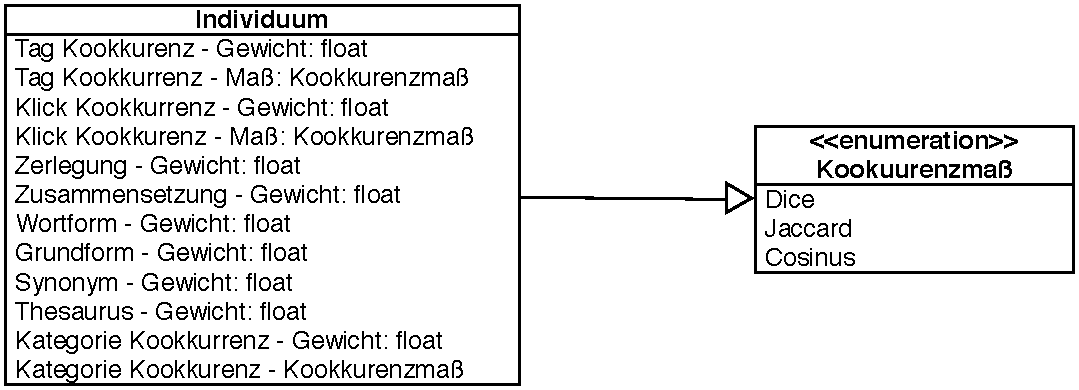
\includegraphics[width=0.9\textwidth]{genotype}
\caption{UML--Klassendiagramm des gewählten Genotyps}
\label{fig:genotype}
\end{figure}

Die reellwertigen Attribute stellen ein Gewicht des jeweiligen Kantentyps dar. Sie können nur relativ zu den anderen Kantengewichten betrachtet werden und somit nur im Rahmen der Optimierung von Interesse. Der Wertebereich dieser Attribute wird auf das Intervall \((0,1)\) eingeschränkt. Die Kookkurrenzmaße entsprechen den in Abschnitt \ref{measures} genannten, also \emph{Dice}, \emph{Jaccard} und \emph{Kosinus}. Der Genotyp ist in Abbildung \ref{fig:genotype} als UML-Klassendiagramm und in Listing \ref{lst:genotyope} beispielhaft in JSON-Notation dargestellt.

\begin{lstlisting}[language=json, label={lst:genotyope}, caption={Beispiel für ein Individuum}]
{
    "tagCoOccMeasure" : 0,
    "tagCoOccWeight" : 0.6878115427680314,
    "clickCoOccMeasure" : 2,
    "clickCoOccWeight" : 0.1533144270069897,
    "synonymWeight" : 0.2355003503616899,
    "thesaurusWeight" : 0.9918724503368139,
    "baseformWeight" : 0.2843543488997966,
    "wordformWeight" : 0.93317318148911,
    "sharedDomainsMeasure" : 2,
    "sharedDomainsWeight" : 0.462230023695156,
    "compositionWeight" : 0.07963851140812039,
    "decompositionWeight" : 0.4740817183628678
}
\end{lstlisting}

\subsection{Initialisierung}

Im Initialisierungsschritt wird die anfängliche Population für jede der Stichproben gebildet. Dazu muss zuerst eine geeignet erscheinende Populationsgröße festgelegt werden.

In jeder Generation müssen im Evaluierungsschritt alle Individuen bewertet werden. Wie einführend bereits erläutert wurde, kann dies nur mit menschlicher Interaktion erfolgen. Somit sollte die Populationsgröße möglichst gering sein, um mit der gleichen Anzahl Bewertungen eine größere Anzahl von Generationen zu durchlaufen. Dies geschieht auf Kosten der Diversität in der Population. Jedoch wurde im Rahmen dieser Arbeit dieser Ansatz gewählt, um möglichst viele Möglichkeiten zu haben, die Parameter zu optimieren.

Es wurde eine Populationsgröße von zehn Individuen je Stichprobe gewählt. Somit müssen in jeder Generation einhundertfünfzig Individuen bewertet werden. Bei der Initialisierung wurden die Variablen jedes erzeugten Individuums zufällig gewählt.

\subsection{Selektion}

Die Bestimmung einer Fitnessfunktion für die Optimierung der Link Discovery gestaltet sich durch die Notwendigkeit menschlicher Beurteilung als schwierig. Eine solche Fitnessbestimmung müsste derart erfolgen, dass ein Benutzer jedem Individuum einen reellwertigen Fitnesswert zuweist. Dies gestaltet ist jedoch auf Grund der hohen Anzahl von Individuen nicht praktikabel.

Jedoch ist das menschliche Eingreifen zwingend notwendig, weshalb es sich beim implementierten Algorithmus um einen \emph{interaktiven} evolutionären Algorithmus \cite{ht2001} handelt. Die interaktive Komponente ist hierbei die Selektion, wodurch der Schritt der Evaluation übersprungen werden kann. Wird die Selektion direkt vom Benutzer ausgeführt, erübrigt sich die Bestimmung eines Fitnesswertes.

Die umgesetzte Selektion erfolgt durch die Durchführung von Wettkämpfen. Hierzu werden in jeder Generation je fünf Paare von Individuen gebildet. Diese Paarungen stellen die Wettkämpfe dar, bei denen der Benutzer den Gewinner bestimmt. Alle Gewinner werden selektiert und im Reproduktionsschritt weiter verwendet.

Der Vorteil dieses Vorgehens ist, dass der Benutzer nur jeweils zwei Lösungskandidaten vergleichen muss, anstatt direkt fünf der zehn Individuen auszuwählen. Somit verringert sich der zu einem Zeitpunkt zu leistende kognitive Aufwand für die Selektion.

\begin{figure}
\centering
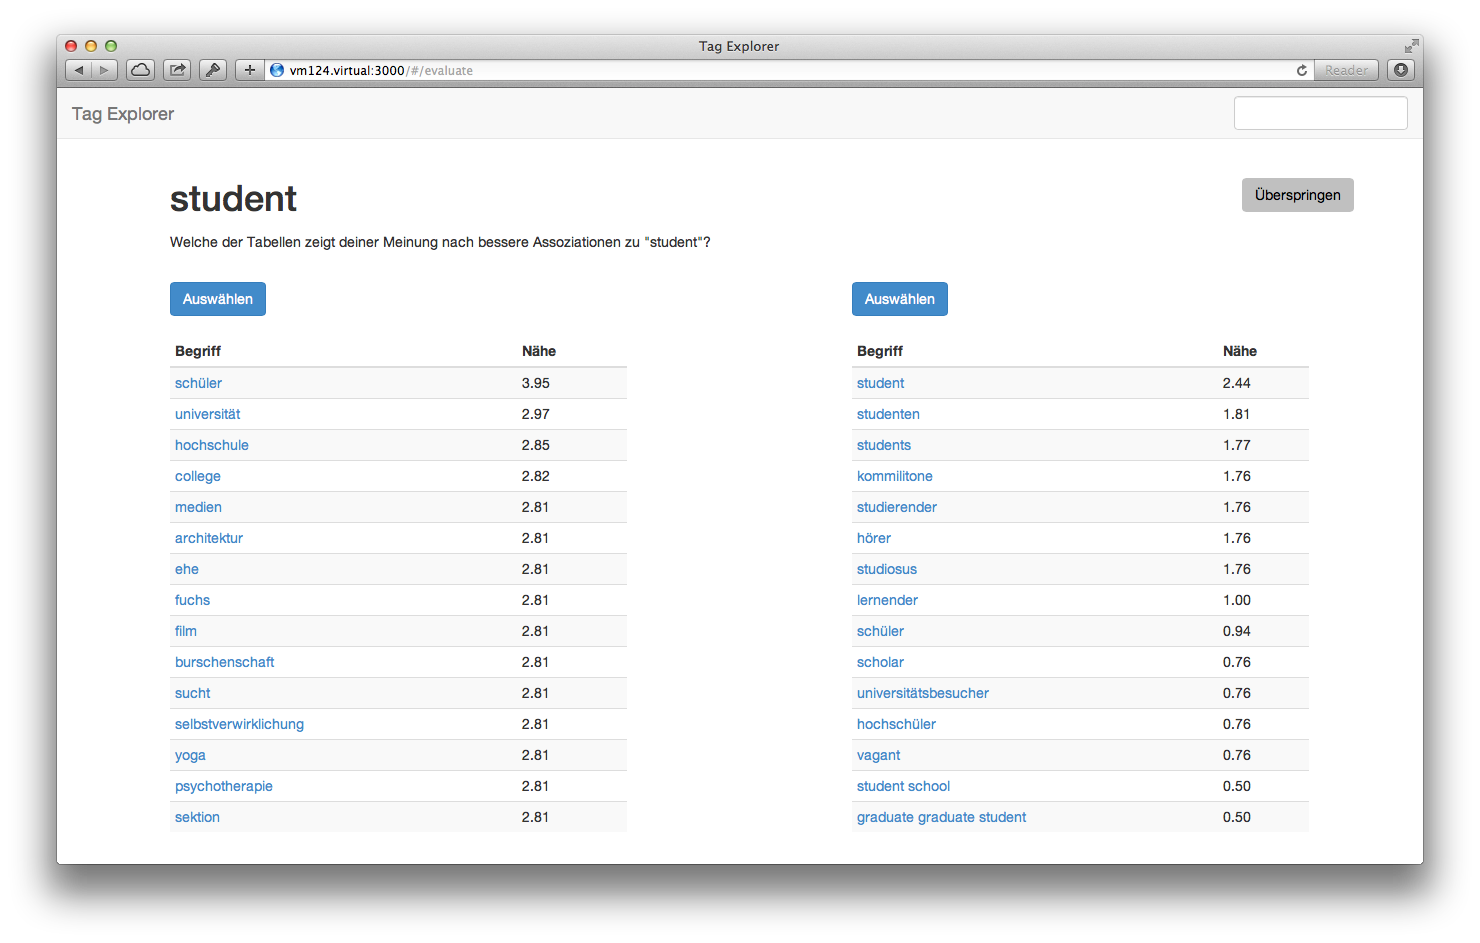
\includegraphics[width=\textwidth]{eva_interface}
\caption{Oberfläche zur interaktiven Selektion}
\label{fig:eva_interface}
\end{figure}

Zur Selektion besucht der Benutzer eine Website, auf der ihm zwei Lösungskandidaten für eine Stichprobe präsentiert werden. Die Lösungskandidaten werden in Form von Listen von je fünfzehn Begriffen dargestellt, die die mit der jeweiligen Kantengewichtung erzeugten nächsten Nachbarn des Begriffes sind. Diese Oberfläche ist in Abbildung \ref{fig:eva_interface} als Screenshot abgebildet. Nach Auswahl eines Gewinners wird dem Nutzer der nächste Wettkampf präsentiert.

Am Selektionsprozess kann sich jeder interessierte Benutzer beteiligen. Dieses Vorgehen wurde gewählt, um ein möglichst breites Spektrum an Meinungen bezüglich der Güte der Verbindungen zu erhalten.

Durch die direkte Auswahl beträgt die Reproduktionswahrscheinlichkeit für die ausgewählten Individuen eins und für die nicht ausgewählten Individuen Null \cite{sd2012}. Die gewählten Reproduktionsverfahren werden im nächsten Abschnitt beschrieben.

\subsection{Reproduktion}

Die fünf selektierten Individuen werden zur Reproduktion herangezogen, um fünf neue Individuen zu erzeugen, damit die Populationsgröße für die nächste Selektion wieder auf zehn Individuen steigt. Dazu werden die selektierten Individuen zuerst rekombiniert, um fünf Kindindividuen zu erzeugen, welche dann durch Mutation verändert werden.

\paragraph{Rekombination}

Als Verfahren zur Rekombination wurde der \emph{Ein-Punkt-Crossover} \cite{kw2007} gewählt. Dazu werden zufällig zwei Elternindividuen ausgewählt und ein zufälliger Crossover-Punkt berechnet. Werden die Genotypen der beiden Elternindividuen als Arrays dargestellt, werden bis zum Crossover-Punkt die Variablen des ersten Individuums, nach dem Crossover-Punk die Variablen des zweiten Individuums übernommen. Der Crossover ist in Abbildung \ref{fig:crossover} dargestellt.

\begin{figure}
\centering
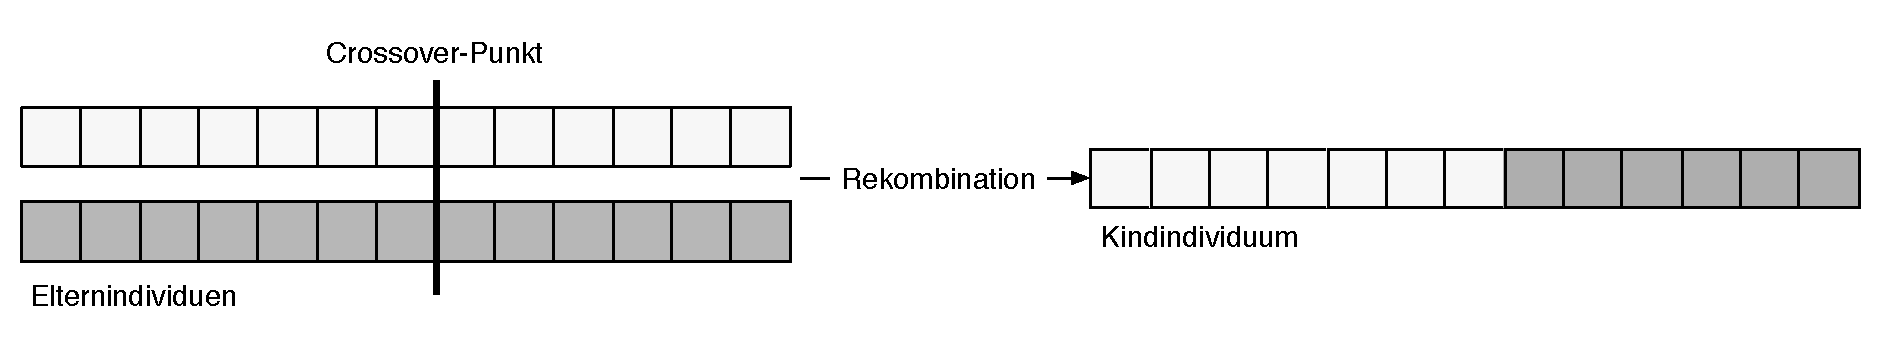
\includegraphics[width=\textwidth]{crossover}
\caption{Ein-Punkt-Crossover}
\label{fig:crossover}
\end{figure}

\paragraph{Mutation}

Zur Mutation der reellwertigen Kantengewichtungen wurde das Verfahren der \emph{Gauß-Mutation} \cite{kw2007} gewählt. Dabei wird zu jeder reellwertigen Variablen des Genotyps ein normalverteilter Zufallswert addiert. Verlässt der entstehende Wert das zulässige Intervall, so wird er auf die entsprechende Intervallschranke angepasst. Die Gauß-Mutation macht daher große Änderungen der Variable möglich, aber weniger Wahrscheinlich als kleine Änderungen. Sie eignet sich somit gut, um Diversität in der Population zu erzeugen. Konkret wurde in der Umsetzung der Optimierung eine auf das Intervall \((0,1)\) angepasste Normalverteilung mit Erwartungswert \(\mu=0\) und Varianz \(\sigma=0.5\) gewählt. Die Variablen für die Kookkurrenzmaße werden nicht mutiert.

Nachdem in diesem Abschnitt die konkrete Umsetzung der Optimierung mittels interaktiver evolutionärer Algorithmen beschrieben wurde, folgt im nächsten Abschnitt die Darstellung und Diskussion der Ergebnisse.

\section{Ergebnisse}

Die Optimierung wurde über insgesamt \num{13} Generationen durchgeführt. Somit wurden über alle Stichproben hinweg \num{975} Selektionen von Benutzern vorgenommen. Die Benutzer waren allesamt Mitarbeiter von Spreadshirt. Aufgrund der anonymen Teilnahme lässt sich nicht angeben, wie viele Einzelpersonen an der Optimierung teilgenommen haben.

\subsection{Kantengewichte}

Da nach jeder Selektion je Stichprobe fünf Individuen in der Population verbleiben, werden zunächst deren Kantengewichtungen untersucht. Tabelle \ref{tab:winners_total} zeigt für jede Variable aus dem Genotyp den Median der in der dreizehnten Generation selektierten Individuen. Das Kantengewicht für den Typ \emph{Zerlegung} ist nicht in der Tabelle enthalten, da es sich bei den Stichproben nur um Einzelwörter handelt.

\begin{table}
\centering
\begin{tabular}{lcccccccc}
    \toprule
    Stichprobe & \(k_t\) & \(k_{kl}\) & \(s\) & \(t\) & \(g\) & \(w\) & \(k_{ka}\) & \(zu\) \\
    \midrule
    Dubstep & 0.85 & 0.60 & 0.53 & 0.77 & 1.00 & 1.00 & 1.00 & 0.48 \\
    Hammer & 0.81 & 0.56 & 0.88 & 0.45 & 1.00 & 0.89 & 0.00 & 0.59 \\
    Kind & 0.58 & 0.22 & 0.84 & 1.00 & 0.66 & 0.00 & 0.01 & 0.00 \\
    Kopfkissenbezug & 0.34 & 0.00 & 0.00 & 0.60 & 0.77 & 0.93 & 0.26 & 0.93 \\
    Krankenschwester & 1.00 & 0.20 & 0.28 & 0.60 & 0.70 & 0.88 & 0.59 & 0.33 \\
    Leipzig & 0.69 & 1.00 & 0.66 & 0.01 & 0.41 & 0.00 & 0.17 & 1.00 \\
    Marathon & 0.62 & 0.70 & 0.23 & 0.41 & 0.69 & 1.00 & 0.00 & 0.95 \\
    Minecraft & 0.71 & 0.34 & 0.31 & 0.38 & 0.74 & 1.00 & 0.00 & 1.00 \\
    Mountainbike & 0.34 & 0.48 & 0.00 & 0.00 & 1.00 & 1.00 & 0.85 & 0.00 \\
    Polska & 0.63 & 0.25 & 0.86 & 0.97 & 0.24 & 1.00 & 0.00 & 0.00 \\
    Regenbogen & 1.00 & 0.43 & 0.36 & 0.47 & 0.00 & 0.26 & 0.61 & 0.52 \\
    Student & 0.67 & 0.15 & 0.38 & 0.84 & 0.78 & 0.70 & 0.72 & 0.33 \\
    Valentinstag & 1.00 & 0.44 & 0.80 & 0.24 & 0.53 & 0.58 & 0.70 & 1.00 \\
    Volkswagen & 0.47 & 1.00 & 0.11 & 0.51 & 1.00 & 0.89 & 0.14 & 0.30 \\
    Wow & 0.08 & 1.00 & 0.93 & 0.21 & 1.00 & 0.54 & 0.53 & 0.68 \\
    \bottomrule
\end{tabular}
\caption{Mediane der Kantengewichte nach der finalen Selektion}
\caption*{
    \begin{tabular}{ll}
        \(k_t\) & Tag-Kookkurrenz\\
        \(k_{kl}\) & Klick-Kookkurrenz\\
        \(s\) & Synonyme \\
        \(t\) & Thesaurus \\
        \(g\) & Grundform \\
        \(w\) & Wortform \\
        \(k_{ka}\) & Kategorie-Kookkurrenz\\
        \(zu\) & Zusammensetzung\\
    \end{tabular}
}
\label{tab:winners_total}
\end{table}

Bei Betrachtung dieser Ergebnisse fällt auf, dass sich die Gewichtungen der Kanten von Stichprobe zu Stichprobe stark unterscheiden. Somit bestätigt sich die Vermutung, dass eine globale Optimierung der Kantengewichtungen keine sinnvollen Ergebnisse erzielt. Jedoch ergaben sich für die Typen \emph{Wortform} und \emph{Grundform} in allen Stichproben relativ hohe Gewichte.



\subsection{Kookkurrenzmaße}

In Tabelle \ref{tab:measures_each} sind für alle Stichproben die nach der letzten Selektion jeweils am häufigsten in der Population auftretenden Kookkurrenzmaße aufgeführt.

\begin{table}
\centering
\begin{tabular}{llll}
    \toprule
    Stichprobe & Tags & Klicks & Kategorien \\
    \midrule
    Dubstep & Jaccard & Dice & Dice \\
    Hammer & Dice & Dice & Kosinus \\
    Kind & Kosinus & Dice & Kosinus \\
    Kopfkissenbezug & Dice & Dice & Kosinus \\
    Krankenschwester & Jaccard & Dice & Dice \\
    Leipzig & Jaccard & Jaccard & Kosinus \\
    Marathon & Dice & Dice & Jaccard \\
    Minecraft & Dice & Dice & Kosinus \\
    Mountainbike & Kosinus & Jaccard & Jaccard \\
    Polska & Jaccard & Dice & Kosinus \\
    Regenbogen & Dice & Dice & Jaccard \\
    Student & Dice & Dice & Dice \\
    Valentinstag & Dice & Jaccard & Kosinus \\
    Volkswagen & Kosinus & Dice & Dice \\
    Wow & Jaccard & Dice & Dice \\
    \bottomrule
\end{tabular}
\caption{Häufigste Kookkurrenzmaße nach der finalen Selektion}
\label{tab:measures_each}
\end{table}